% !TEX program = pdflatex
\RequirePackage[l2tabu, orthodox]{nag}
\documentclass{article}

% FONTS
\usepackage[T1]{fontenc}

% Replace default Latin Modern typewriter with its proportional counterpart
% http://www.tug.dk/FontCatalogue/lmoderntypewriterprop/
\renewcommand*\ttdefault{lmvtt}


%%% OPTION 1 - Fourier Math + New Century Schoolbook + ParaType Sans

% % Import Fourier Math (this imposes its own New Century Schoolbook type)
% % http://www.ctan.org/tex-archive/fonts/fouriernc/
% \usepackage{fouriernc}
% \usepackage{amsmath}
% % Replace with TeX Gyre Schola version of New Century Schoolbook (must scale!)
% % http://www.tug.dk/FontCatalogue/tgschola/
% \usepackage[scale=0.92]{tgschola}
% \usepackage[scaled=0.88]{PTSans}

%% OPTION 2 - MathDesign Math + Bitstream Charter + ParaType Sans

% Import MathDesign (this brings along Bitstream Charter)
% http://www.ctan.org/tex-archive/fonts/mathdesign/
\usepackage[bitstream-charter]{mathdesign}
\usepackage{amsmath}
\usepackage[scaled=0.92]{PTSans}


% %%% OPTION 3 - MTPRO 2 Math + Termes Times + ParaType Sans

% \usepackage{tgtermes}
% \usepackage{amsmath}
% \usepackage[subscriptcorrection,
%             amssymbols,
%             mtpbb,
%             mtpcal,
%             nofontinfo  % suppresses all warnings
%            ]{mtpro2}
% \usepackage{scalefnt,letltxmacro}
% \LetLtxMacro{\oldtextsc}{\textsc}
% \renewcommand{\textsc}[1]{\oldtextsc{\scalefont{1.10}#1}}
% \usepackage[scaled=0.92]{PTSans}

% GEOMETRY
\usepackage[
  paper  = letterpaper,
  left   = 1.65in,
  right  = 1.65in,
  top    = 1.0in,
  bottom = 1.0in,
  ]{geometry}

% COLOR
\usepackage[usenames,dvipsnames]{xcolor}
\definecolor{shadecolor}{gray}{0.9}

% SPACING and TEXT
\usepackage[final,expansion=alltext]{microtype}
\usepackage[english]{babel}
\usepackage[parfill]{parskip}
\usepackage{afterpage}
\usepackage{framed}

%redefine the leftbar environment to accept a width and coloring options
\renewenvironment{leftbar}[1][\hsize]
{%
  \def\FrameCommand
  {%
    {\color{Gray}\vrule width 3pt}%
    \hspace{10pt}%
    %\hspace{0pt}\fboxsep=\FrameSep\colorbox{black!10}%
  }%
  \MakeFramed{\hsize#1\advance\hsize-\width\FrameRestore}%
}%
{\endMakeFramed}

% define a paragraph header function
\DeclareRobustCommand{\parhead}[1]{\textbf{#1}~}

% EDITING
% line numbering in left margin
\usepackage{lineno}
\renewcommand\linenumberfont{\normalfont
                             \footnotesize
                             \sffamily
                             \color{SkyBlue}}
% ragged paragraphs in right margin
\usepackage{ragged2e}
\DeclareRobustCommand{\sidenote}[1]{\marginpar{
                                    \RaggedRight
                                    \textcolor{Plum}{\textsf{#1}}}}
% paragraph counter in right margin
\newcommand{\parnum}{\bfseries\P\arabic{parcount}}
\newcounter{parcount}
\newcommand\p{%
    \stepcounter{parcount}%
    \leavevmode\marginpar[\hfill\parnum]{\parnum}%
}
% paragraph helper
\DeclareRobustCommand{\PP}{\textcolor{Plum}{\P} }

% COUNTERS
\renewcommand{\labelenumi}{\color{black!67}{\arabic{enumi}.}}
\renewcommand{\labelenumii}{{\color{black!67}(\alph{enumii})}}
\renewcommand{\labelitemi}{{\color{black!67}\textbullet}}

% FIGURES
\usepackage{graphicx}
\usepackage[labelfont=bf]{caption}
\usepackage[format=hang]{subcaption}

% TABLES
\usepackage{booktabs}

% ALGORITHMS
\usepackage[algoruled]{algorithm2e}
\usepackage{listings}
\usepackage{fancyvrb}
\fvset{fontsize=\normalsize}

% BIBLIOGRAPHY
\usepackage{natbib}

% HYPERREF
\usepackage[colorlinks,linktoc=all]{hyperref}
\usepackage[all]{hypcap}
\hypersetup{citecolor=BurntOrange}
\hypersetup{linkcolor=MidnightBlue}
\hypersetup{urlcolor=MidnightBlue}

% CLEVEREF must come after HYPERREF
\usepackage[nameinlink]{cleveref}

% ACRONYMS
\usepackage[acronym,smallcaps,nowarn]{glossaries}
% \makeglossaries

% COLOR DEFINITIONS
\newcommand{\red}[1]{\textcolor{BrickRed}{#1}}
\newcommand{\orange}[1]{\textcolor{BurntOrange}{#1}}
\newcommand{\green}[1]{\textcolor{OliveGreen}{#1}}
\newcommand{\blue}[1]{\textcolor{MidnightBlue}{#1}}
\newcommand{\gray}[1]{\textcolor{black!60}{#1}}

% LISTINGS DEFINTIONS
\lstdefinestyle{mystyle}{
    commentstyle=\color{OliveGreen},
    keywordstyle=\color{BurntOrange},
    numberstyle=\tiny\color{black!60},
    stringstyle=\color{MidnightBlue},
    basicstyle=\ttfamily,
    breakatwhitespace=false,
    breaklines=true,
    captionpos=b,
    keepspaces=true,
    numbers=left,
    numbersep=5pt,
    showspaces=false,
    showstringspaces=false,
    showtabs=false,
    tabsize=2
}
\lstset{style=mystyle}


\DeclareRobustCommand{\mb}[1]{\ensuremath{\boldsymbol{\mathbf{#1}}}}

\DeclareMathOperator*{\argmax}{arg\,max}
\DeclareMathOperator*{\argmin}{arg\,min}

\DeclareRobustCommand{\KL}[2]{\ensuremath{\textrm{KL}\left(#1\;\|\;#2\right)}}

\newcommand{\mbx}{\mathbold{x}}
\newcommand{\mbX}{\mbf{X}}

\newcommand{\mbz}{\mathbold{z}}

\newcommand{\mbI}{\mbf{I}}

\newcommand{\mbZ}{\mbf{Z}}
\newcommand{\mbL}{\mbf{L}}

\newcommand{\mbtheta}{\mathbold{\theta}}
\newcommand{\mbTheta}{\mathbold{\Theta}}
\newcommand{\mbomega}{\mathbold{\omega}}
\newcommand{\mbOmega}{\mathbold{\Omega}}
\newcommand{\mbsigma}{\mathbold{\sigma}}
\newcommand{\mbSigma}{\mathbold{\Sigma}}

\newcommand{\mblambda}{\mathbold{\lambda}}
\newcommand{\mbgamma}{\mathbold{\gamma}}
\newcommand{\mbzeta}{\mathbold{\zeta}}
\newcommand{\mbeta}{\mathbold{\eta}}
\newcommand{\mbbeta}{\mathbold{\beta}}
\newcommand{\mbphi}{\mathbold{\phi}}
\newcommand{\mbmu}{\mathbold{\mu}}
\newcommand{\mbrho}{\mathbold{\rho}}

\newcommand\dif{\mathop{}\!\mathrm{d}}
\newcommand{\diag}{\textrm{diag}}
\newcommand{\supp}{\textrm{supp}}

\newcommand{\E}{\mathbb{E}}
\newcommand{\Var}{\mathbb{V}\textrm{ar}}

\newcommand{\bbN}{\mathbb{N}}
\newcommand{\bbZ}{\mathbb{Z}}
\newcommand{\bbR}{\mathbb{R}}
\newcommand{\bbS}{\mathbb{S}}

\newcommand{\cL}{\mathcal{L}}

\newcommand{\cN}{\mathcal{N}}
\newcommand{\Gam}{\textrm{Gam}}
\newcommand{\InvGam}{\textrm{InvGam}}

\newacronym{KL}{kl}{Kullback-Leibler}
\newacronym{ELBO}{elbo}{\emph{evidence lower bound}}
\newacronym{POPELBO}{pop-elbo}{\emph{population evidence lower bound}}

\newacronym{SVI}{svi}{stochastic variational inference}
\newacronym{BUMPVI}{bump-vi}{bumping variational inference}

\newacronym{GMM}{gmm}{Gaussian mixture model}
\newacronym{LDA}{lda}{latent Dirichlet allocation}

\newacronym{SUTVA}{sutva}{stable unit treatment value assumption}


\DeclareMathOperator*{\tr}{tr}

\newcommand{\UN}[1]{\ensuremath{\left|#1\right|_\infty}}
\newcommand{\EN}[1]{\ensuremath{\left|#1\right|}}
\newcommand{\kldiv}[2]{\ensuremath{D\left(#1||#2\right)}}

\usepackage{cancel}

% \linenumbers

\title{Markov Link Method for calibrating without joint measurement, including the case of destructive measurements}
\author{Jackson Loper}

\usepackage{amsthm}
\newtheorem*{thm}{Theorem}
\newtheorem{lem}{Lemma}
\newtheorem{conj}{Conjecture}

\theoremstyle{definition}
\newtheorem{example}{Example}

\begin{document}
\maketitle

\begin{abstract}
A proliferation of new experimental tools has left a serious gap: calibration. Two thermometers can be calibrated against each other by simply measuring the same bodies of water with both thermometers, but the problem is much harder for many modern tools.  One common problem is that we do not have measurements from the same ``body of water'' for both tools.  We propose the Markov Link Method (MLM) as a way to overcome this difficulty.   This method produces consistent estimators that tightly bound the calibration, i.e. the conditional distribution of one tool's measurement given another tool's measurement. It achieves this without any measurement data from both tools applied to the same ``bodies of water.'' Moreover, MLM makes zero assumptions about what calibrations we might expect to see, instead applying a subpopulation-based conditional independence assumption.   We evaluate MLM on a pair of single-cell RNA techniques, obtaining precise calibrations between the tools as well as more accurate models for each tool separately.
\end{abstract}

The modern setting is rife with experimental measurement tools, and it can be very frustrating to understand how the output of these tools relate to one another.  This problem is known as ``calibration'' or ``zeroing'' \cite{bipm2008international}.  A calibration tells us what readings we should expect from one tool, given the reading we obtained from another tool.   Calibration additionally must give uncertainty bounds for how much we can trust those expectations.  Calibration between measurement tools allows us to combine experimental results from different labs and different methodologies into larger scientific theories.  

Formally, a calibration is simply a conditional distribution.  We will denote it by $q^*(y|x)$.  As input, this conditional distribution takes the measurement results from one tool on a particular specimen, $x$.  As output, it yields the probability of obtaining result $y$ from a second tool applied to measure the same specimen.  One way to learn the calibration is to measure the same specimens under both tools.  We call this ``joint measurement.''  Unfortunately, calibrations are often required even when joint measurement is unavailable.  For example, if the measurement tool alters the specimen being measured, joint measurement is simply impossible.  In other cases, it may be expensive or impractical.

We here propose the Markov Link Method (MLM) to estimate calibrations between tools.  The MLM can be trained without any joint measurement.  The key idea is to use multiple subpopulations of specimens.  If each subpopulation captures a different slice of the overall population, we can obtain tight bounds on the true calibration.  This is true even if each subpopulation is highly heterogeneous.  By integrating information from all the subpopulations we can make rigorous deductions about what the calibration might be.  MLM also gives suggestions about which further subpopulations might be helpful to study in order to further refine our knowledge of the true calibration.  The method can also be naturally extended to calibration distributions among many tools.

\section{The Markov Link Method assumption}

To make these ideas rigorous, let us develop a little bit of notation.  Let us say we are considering the members of a large population.  For example, each ``specimen`` in the large population might be a human cell or a piece of metal which needs to be tested.  We will assume there are three basic properties of interest for each specimen $i$:

\begin{enumerate}
\item $\ell_i$, the subpopulation or side information.  We assume that the overall population can be split into subpopulations of interest.  For example, we could define subpopulations by looking at cells in different parts of the body, or cells with different sizes.  
\item $X_i$, the result of measuring a specimen with tool I.  For example, perhaps tool I takes a picture of the cell with a destructive electron microscopy method.
\item $Y_i$, the result of measuinrg a specimen with tool II.  For example, perhaps tool II measures the RNA expression of the cell with a destructive sequencing method.
\end{enumerate}

We here consider the case that ``joint measurement'' is impossible or impractical.  In terms of the notation above, that means that for any given specimen we can either observe $\ell_i, X_i$ or $\ell_i,Y_i$.  We can never observe $\ell_i,X_i,Y_i$ for any specimen $i$.  Despite this obstacle, we would like to estimate the conditional distribution $q^*(y|x)\triangleq \mathbb{P}(Y_i=y|X_i=x)$.  Under suitable assumptions, we will see that such estimation is indeed possible using the side information $\ell$.  However, this estimation suffers from so-called \emph{identifiability problems}, which we will describe in detail in the next section.  Fortunately, this identifiability error can be quantified, allowing us to determine exactly what our data tells us about the true calibration.  If the identifiability error is large, the Markov Link method suggests future experiments based on new subpopulations which will hone down on the identifiability problem.

\begin{figure}
\hfill{}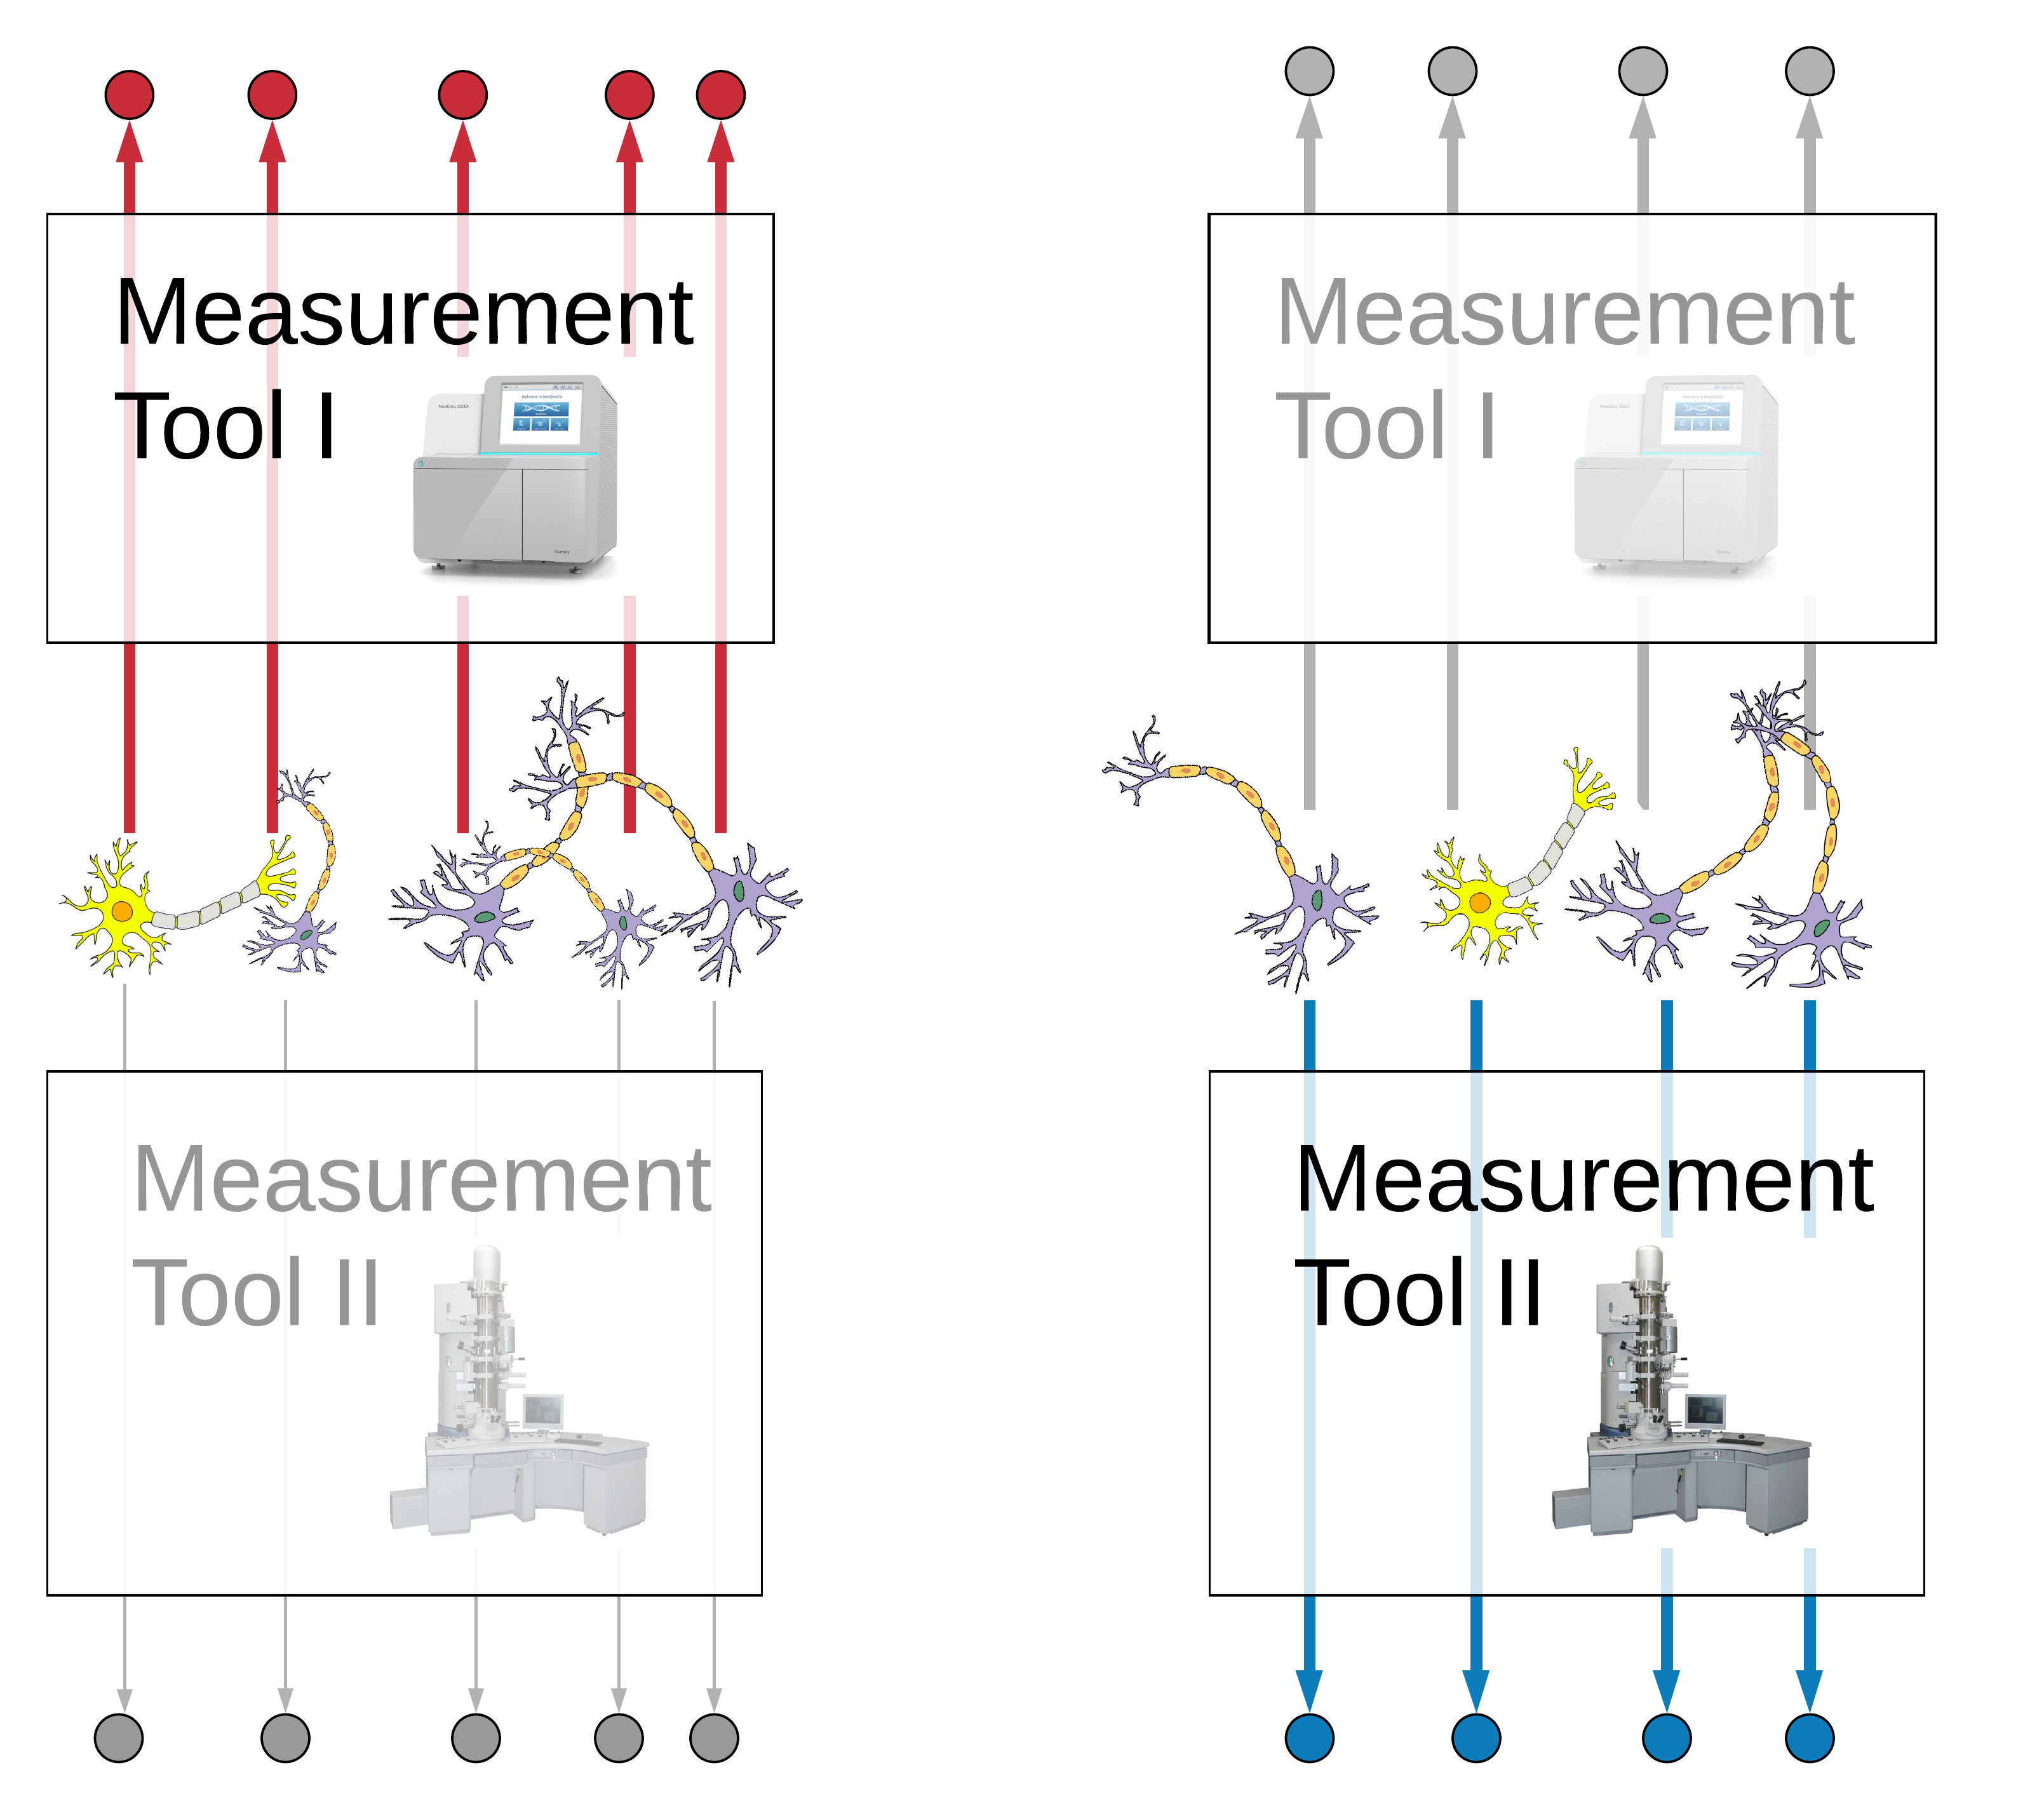
\includegraphics[width=.7\textwidth]{../images/bigpicture}\hfill{}
\caption{We consider the case that for each specimen there are two ways we might measure it.  We divide the specimens into two groups.  The specimens on the left are measured with technique I and the specimens on the right are measured with technique II.  In the end, we are left wondering: what would have happened if we had measured the specimens on the left with technique II?  Or what if we had measured the specimens on the right with technique I?  The Markov Link Method gives a way to answer this problem using a subpopultaion analysis.  For each specimen, we take $\ell$ to indicate the subpopulation (indicated here by the color of the neuron, i.e.\ yellow or purple), $X$ to indicate the results we would obtain from that specimen if we measured it with method I, and $Y$ to indicate the results we would obtain from that specimen if we meausured it with method II. \label{fig:bigpicture}}
\end{figure}

The key assumption of the Markov Link Method is a conditional independence assumption: that $\mathbb{P}(Y|X,\ell_i)$ is independent of $\ell$, i.e. $\mathbb{P}(Y=y|X=x,\ell)=q^*(y|x)$ for every value of $\ell$.  Intuitively, this signifies that the manner in which $X$ and $Y$ are related is the same for each subpopulation.  If this assumption is not met, then the method presented here is not applicable.  The validity of these assumptions for a given situation should be closely contemplated.  

Let us consider a few real-world examples where this assumption may apply.

\begin{itemize}
    \item Quality control for manufacturing.   The surest way to test the reliability of a part is to construct a machine that pushes the part until it breaks.  However, how can we test the reliability of the machine that performs the test?  In each test run there will be some variability induced by the machine itself, which induces a measurement error  In practice, some kind of assumptions about part homogeneity are used to approximate this error (cf.\ \cite{de2005gauge}).  However, if we have two testing machines we can use the MLM to obtain a calibration between the machines, even though we can never test the same part with both machines.  This enables us to bound the overall measurement error.  In this case, $\ell$ might indicate the type of a part being tested, $X$ would indicate the reliability of a part as measured by one machine, and $Y$ would indicate the reliability of a part as measured by another machine.  If the error in machine $Y$ is not correlated to the part type $\ell$, then the MLM assumption certainly holds.  Even if the error is correlated, the MLM assumption may still hold.  For example, imagine that the $Y$ error is correlated with the absolute reliability of the part, this may pose no problem because that reliability is measured by $X$.  As long as the correlations are the result of something which is measured in $X$, the conditional independence assumption will hold.  

    \item Combining knowledge across experimental modalities: morphology and transcriptomics.  There are different ways to think about the different types of cells in an organism.  A traditional approach is to classify cells based on what they look like (cf.\ \cite{steinman1973identification,bloomfield1982physiological}).  A more modern approach is to assay the cell's transcriptome (cf.\ \citep{tasic2017shared}).  Unfortunately, modern high-resolution cell photography and single-cell sequencing technologies are both destructive.  As a result, we can't get both kinds of data for the same specimens.  For cells native to regions full of diverse cell-types, finding a correspondence is a real problem.  The result is two completely independent classifications of cells, one for each way of looking at the cell.  MLM allows us to estimate the relationship between those two classification systems, yielding a wholistic understanding of the different types of cells.  In this case, $\ell$ might indicate some side information such as where in the body the cell was found, $X$ would indicate the classification of the cell according to its transcriptomics, and $Y$ would indicate the classification of a cell according to its morphology.  We expect that cell morphology is largely a function of cell transcriptomics.  Thus, as long as the $X$ measurement is sufficiently detailed, we expect that any correlations between $Y$ and $\ell$ would be explained by $X$.  That is, the MLM assumption holds.  
 
    \item Cancer treatment efficacy prediction.  Starting from in-vivo human cancers, many cell-lines have been cultured over the years.  These cell cultures live indefinitely on plates.  Many experiments have been performed to see how these cancer cells respond to treatment.  However, if a treatment work on a particular cultured cell-line, what can we say about which kinds of cancer might respond well to that treatment?  Coarse side-information such as original cancer location is often available for both in-vivo and cultured cells, but this is often a surprisingly weak signal.  Cell transcriptomes provides much more specific information about the cancer, and thus, in theory, what treatments might be appropriate (cf.\ \cite{cieslik2018cancer}).  However, we know that cultured cell-lines look quite different from in-vivo cells (cf. \cite{imamura2015comparison,haibe2013inconsistency}).  Moreover, we have very little joint measurement between the human cells which originally gave rise to a cell culture and the cells that survived to beceome the cell line.  The Markov Link method can leverage the common side-information together with separate transcriptome information to produce a fine-grained correspondence between in-vivo and cultured cells.  This correspondence can used to propose new treatments for cancers.  Here $\ell$ might indicate cancer location, $X$ might indicate transcriptomic expression of cultured cells, and $Y$ might indicate transcriptomic expression of in-vivo cells.  As the transcriptomic expression is much more informative than the cancer location, it is plausible that $X$ might be sufficient to explain any correlations between $\ell$ and $Y$.  Thus the MLM assumption may hold.

    \item Text/image correspondence.  Automatic image captioning is an ongoing effort in machine learning (cf.\ \cite{srivastava2018survey}).  There are three types of data available to help develop such algorithms: text-only data, image-only data, and paired-text-and-image data.  Obviously the last kind is the most useful for automatic image captioning, but there is much less of it.  The Markov Link Method suggests one way to use the more plentiful text-only and image-only data.  We can first apply classic machine learning techniques to get coarse labels for both kinds of data.  Using this side-information to identify subpopulations, the MLM can then deduce a fine-grained correspondence between text and images by combining information from across all the subpopulations.  Here $\ell$ would indicate coarse labels such as ``cat'' or ``street scene.''  These labels could be derived from either images or text and can be trained in a supervised fashion.  Then, $X$ would indicate the image and $Y$ would indicate a caption.  Since the caption should be determined by the picture $X$, the MLM assumption may hold.  

    \item Replication crisis and lab effects.  Replicating a published study is not always an easy thing to do.  This difficulty is commonly attributed to selective publication bias, bad design, poor description of methods, and even outright fraud \cite{baker2016reproducibility}.  A calibration would allow us to understand this problem in detail.  If two labs perform identical experiments and get different data, that does not mean we need to throw out both datasets.  Instead, we can use MLM to calibrate the tools.  Once the tools are properly calibrated, we can combine both datasets.  Unlike other tools to deal with lab or batch effects (e.g. \cite{crow2018characterizing,johnson2007adjusting}), MLM makes zero assumptions about what calibrations we might expect.  In this case, $\ell$ would indicate subpopulations which both labs could access.  For example, we can take several batches of mice; for each batch we can send half to one lab and half to the other lab.  $X$ will the indicate the full results from each specimen examined in one lab and $Y$ coarser information from specimens examined in the other.  If the $X$ data is sufficiently detailed, the MLM assumption may hold.  
\end{itemize}

The main contributions of this paper are summarized here:

\begin{itemize}
\item Posing of the Markov Link Method assumption as an assumption that may make it possible to perform calibrations without joint measurement.
\item An analysis of some identifiability problems posed by the Markov Link Method assumption.  Although it turns out precise identifiability is often impossible, we formulate an asymptotic theory for bounding the magnitude of the this problem.  In particular, although we often cannot hope to exactly determine the calibration $q^*(y|x)\triangleq\mathbb{P}(Y=y|X=x)$, we can estimate a so-called polytope $\hat \Theta$ which captures our uncertainty about $q^*$ due to identifiability problems.
\item The result of the identifiability analysis is a polytope $\hat \Theta$.  We investigate various ways of measuring the extent of this polytope.  We see how it is possible to understand what this ``extent'' means in terms of the identifiability problem.  When the extent is small, we see that the identifiability problem is actually quite minor.
\item We apply the MLM to two single-cell transcriptomic datasets.  The result uncovers an important and unexpected property of one of the experimental methods.  
\end{itemize}

Our identifiability analysis stands on the shoulders of a long history of relating probabilistic assumptions to probabilistic inequalities on unidentifiable parameters.  Indeed, the core idea of this work is to take an assumption (the Markov Link assumption) and use it to place inequality bounds on an unidentifiable quantity (namely $q^*$).  When inequalities are fairly tight on all sides, we see that much can be learned even when what we want isn't identifiable.  Much of the prior literature in this kind of direction comes from research into causality.  For example, in \cite{bonet2001instrumentality} Bonet uses polytopes not unlike the ones seen here to explore whether a variable can be used as an instrument.  The famous Clauser-Horne-Shimony-Holt inequality was designed to help answer causality questions in quantum physics, but it also sheds light on what distributions are consistent with certain assumptions \cite{clauser1969proposed}.  Indeed the physics literature has contributed many key inequalities (cf. \cite{chaves2014inferring}, \cite{kela2017semidefinite}, and the references therein).  Perhaps the closest work to this one would be \cite{makarov1982estimates}, which used two marginal distributions to get bounds on a property of the joint distribution (namely the distribution of the sum).  We advance this approach to a more general-purpose technique, both by using many subpopulations to refine our estimates and by considering the entire space of possible joint distributions instead of simply a particular aspect of the joint.  

The remainder of this work proceeds as follows.  First we give a careful consideration to the Markov Link Method assumption and how it allows us to use side information to estimate the calibration.  We also see when this side information will and will not be helpful.  Next, we outline the Markov Link Method and describe a new asymptotic consistency result concerning the identifiability issues.   Finally, we consider a real dataset.  We perform the method and then attempt to criticize the result three ways: through concerns about not having enough data, through concerns about modeling assumptions, and through concerns about identifiability.  The method largely prevails against these criticisms, and reveals an unexpected feature of the two techniques. 

\section{Precise problem formulation and discussion of the identifiability problem}

Let us now be completely rigorous.  We shall make three assumptions:

\begin{enumerate}
\item For each specimen $i$, the distribution of $X_i,Y_i|\ell_i$ may be written 
\[
\mathbb{P}(X_i=x,Y_i=y|\ell_i) = p^*(x|\ell_i)q^*(y|x)
\]
This is the central assumption we have discussed at length above.  For convenience we will also introduce the notation
\[
\mathbb{P}(Y=y|\ell) = h^*(y|\ell)=\sum_x p^*(x|\ell) q^*(y|x)
\]
\item Joint measurement is unavailable.  In particular, we will assume we have $n+m$ individual specimens.  Of these, we have observed $\ell_i,X_i$ for $i\in\{1\cdots n\}$ and $\ell_i,Y_i$ for $i\in n+1\cdots n+m$.  
\item $X$ and $Y$ are discrete random variables with finite support (the general concepts here will apply more generally, but we leave it for future work).  If the data is not discrete, we can always make it so by dividing it into suitable bins.  In this simple case, we may summarize all of this information with two matrices:
\[
N^X_{\ell x} = |\{i\leq n:\ \ell_i=\ell,X_i=x\}|  \qquad N^Y_{\ell y} = |\{i>n:\ \ell_i=\ell,Y_i=x\}|
\]
Thus $N^X,N^Y$ are matrices counting the number of each kind of observation for method I and method II respectively. 
\end{enumerate}

Our goal will be to use $N^X,N^Y$ to estimate $q^*$, the calibration.  However, \emph{the data from the matrices $N^X,N^Y$ only enable us to estimate $p^*,h^*$}.  They do not enable us to directly estimate $q^*$.  Therefore, we define
\[
\Theta(p,h) \triangleq  \left\{q:\ \sum_x p(x|\ell)q(y|x) = h(y|\ell)\ \forall \ell,y,\ q(y|x)\geq 0\ \forall x,y, \sum_y q_{xy}=1\ \forall x\right\}
\]
as the set of values of the calibration $q$ which are consistent with a given value of $p$ (the conditional distribution of $X|\ell$) and $h$ (the conditional distribution of $Y|\ell$).  Any effort to estimate $q^*$ must therefore overcome two fundamentally different challenges:

\begin{description}
\item[Not-enough-data problems] We don't have infinite data, so we can't hope to exactly determine $p^*,h^*$.
\item[Identifiability problems] Even if we knew $p^*,h^*$ exactly, it is often impossible to know the value of $q^*$.  We can only ever know that it lies somewhere in $\Theta(p^*,h^*)$.  
\end{description}

Let us now take a moment to understand the set $\Theta$.  This set tells us how the things we can estimate (i.e.\ $p^*,h^*$) inform us about what we want to know (i.e.\ $q^*$).  To understand a bit more concretely how this works, it may be helpful to think of $p^*,h^*,q^*$ as matrices.  From this point of view, one aspect of the definition of $\Theta$ can be written more concisely as a matrix equality constraint on $q^*$: if $q \in \Theta(p^*,h^*)$, then $p^*q=h^*$.  The consequences of this equation depend upon whether $p^*$ has a left-pseudoinverse.
\begin{itemize}
    \item If $p^*$ has a left-pseudoinverse then this equation allows us to uniquely determine what we want ($q^*$) in terms of what we know ($p^*,h^*$).  In general, this will happen when the number of subpopulations outnumbers the number of different states that $X$ can take on.  In this case, the problem should be straightforward to solve.   
    \item If $p^*$ does not have a left-pseudoinverse, then there is an identifiability issue: we can never hope to exactly determine $q^*$.  
\end{itemize}

In this paper we will focus almost entirely on the second case.  In this second case there is a genuine identifiability issue;  it is \emph{impossible} to ever determine the true value of $q^*$, regardless of how much data we have.  It therefore becomes of paramount importance to understand the magnitude of this identifiability problem.  In particular, even though we cannot know $q^*$ exactly, can we place bounds on what $q^*$ could be?

To gain intuition, let us consider a few examples.\vspace{.1in}

\begin{example}
Let $\ell \in \{1,2\}$, $X\in \{1,2,3\}$, $Y\in \{1,2\}$, and 
\[
p^{*}=\left(\begin{array}{ccc}
40\% & 50\% & 10\% \\
10\% & 10\% & 80\%
\end{array}\right)\qquad h^{*}=\left(\begin{array}{cc}
20\% & 80\% \\
40\% & 60\%
\end{array}\right)
\]
That is, for example, $p^*_{1,2}=\mathbb{P}(X=2|\ell=1)=50\%$ and $h^*_{2,1}\mathbb{P}(Y=1|\ell=2)=40\%$.  Let us look at a single equation in the system $p^* q^* = h^*$ entailed by the MLM assumption.  For example, $h^*_{2,1}$, we get
\[
0.4 = h^*_{2,1} = \sum_x p^*_{2,x} q^*_{x,1} = .1 q^*_{1,1} + .1 q^*_{2,1} + .8 q^*_{3,1} 
\]
This immediately tells us something about $q^*$.  For example we now know that $q^*_{1,1} = 10(.4 - .1 q^*_{2,1} - 0.8 q^*_{3,1})$.  But it actually tells us much more than that.  Observe that $0\leq q^*_{xy}\leq 1$ for every $x,y$; in other words, probabilities must be positive by definition.  Thus, in particular,
\[
0.4 = .1 q^*_{1,1} + .1 q^*_{2,1} + .8 q^*_{3,1} \leq .2 + .8 q^*_{3,1}
\]
It follows immediately that $q^*_{3,1}\geq .25$.  Each equation in the MLM system yields insights of this kind; together these insights form the constraints that define $\Theta$.  The more different subpopulations you have, the more equations of this kind you will have.  
\end{example}

\vspace{.1in}

\begin{example}
Let $\ell \in \{1\}$, $X\in \{1,2,3,\cdots 11\}$, $Y\in \{1,2\}$, and 
\[
p^{*}=\left(\begin{array}{ccccc}
90\% & 1\% & 1\% & \cdots & 1\% \\
\end{array}\right)\qquad h^{*}=\left(\begin{array}{cc}
95\% & 5\% \\
\end{array}\right)
\]
Here we have only \emph{one} population.  Still we are able to say something quite significant; using similar reasoning to that shown above we see that $q^*_{1,1}\geq 94.\bar4\%$.  
\end{example}

\vspace{.1in}

\begin{figure}
\hfill{}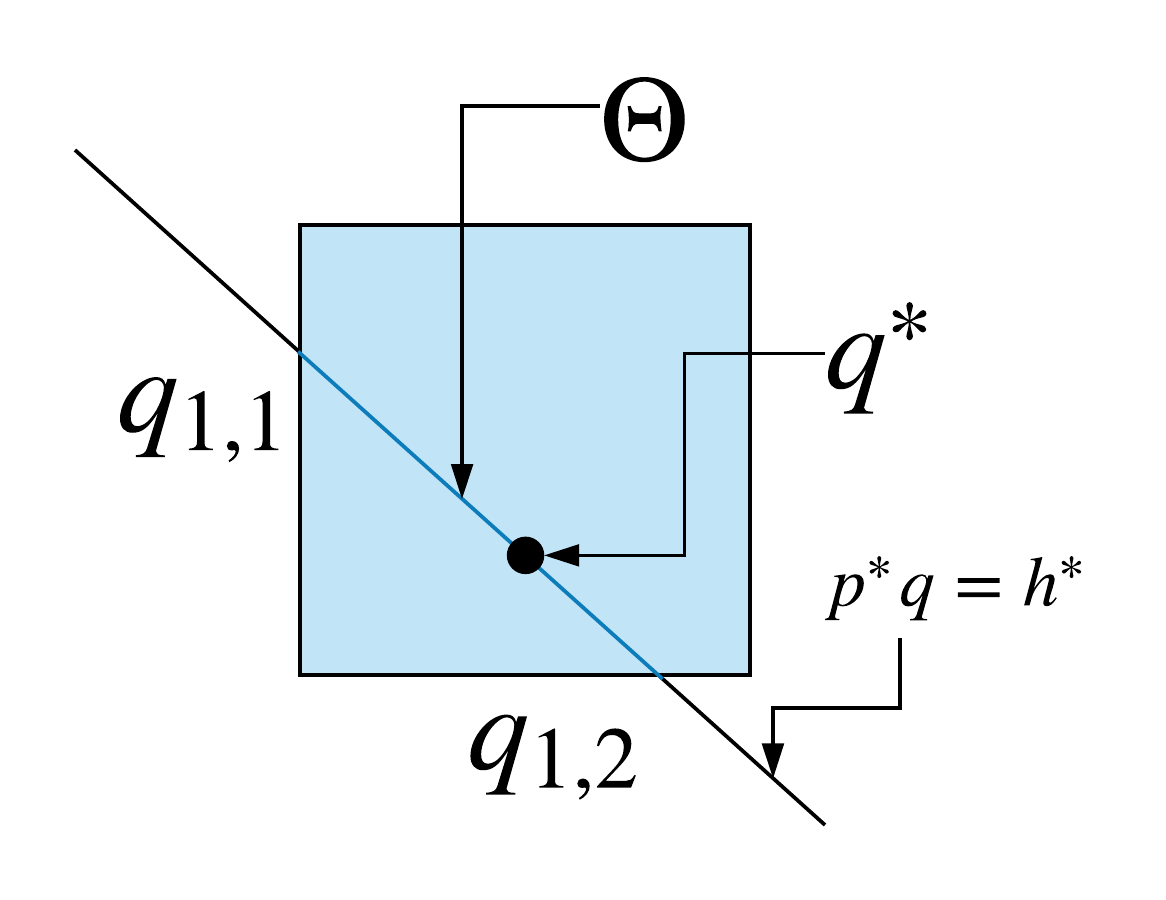
\includegraphics[width=.7\textwidth]{../images/polytope}\hfill{}
\caption{We consider the simple case $\ell=1$, $X\in \{1,2\}$, $Y\in \{1,2\}$.  Then the space of values of $q$ which are valid probability distributions can be understood as a box.  The space of values of $q$ which satisfy the matrix equation $p^* q = h^*$ can be understood as a line that passes through that box.  The set of possible values of $q$ which are consistent with the matrix equation and are also valid probability distributions forms the set $\Theta$, a line segment.  We know that the true value of $q^*$ must lie somewhere inside this $\Theta$.  Depending upon the exact values of $p^*,h^*$, this line segment may be larger or smaller.  For example, if the line crosses close to a corner of the box, then $\Theta$ may be restricted to a very small region near that corner.  \label{fig:polytopeexample}}
\end{figure}

\begin{example}
Finally, let us consider one class of examples in which the entire situation can be visualized: $\ell=1$, $X\in \{1,2\}$, $Y\in \{1,2\}$.   Let $\theta^*_1 = q_^*{1,1}$ and $\theta^*_2 = q_^*{2,1}$.  Notice that in this simple case $\mathbb{P}(Y=2|\ell) = 1- \mathbb{P}(Y=1|\ell)$, so the two values $\theta_^*1,\theta_2^*$ completely define $q^*$.  The matrix equation $p^* q^* = h^*$ corresponds to a linear constraint on $\theta^*$.  On the other hand, the fact that $q^*$ must be a valid probability distribution tells us that $\theta_1^*,\theta_2^*$ must lie inside the box $[0,1]\times[0,1]$.   Combining the matrix equation with the constraints of the box, we learn that $q^*$ lies inside a certain bounded, one-dimensional space.  This space is precisely $\Theta$.  The length of this line segment depends on the exact values of $p^*,h^*$.  In some cases it is quite large, i.e.\ it will be difficult to know much about the true value of $q^*$.  However, in other cases the positivity restrictions force $\Theta$ to be a very small region indeed.  See Figure \ref{fig:polytopeexample} to visualize this.  In general, this $\Theta$ is much higher-dimensional and harder to visualize, but in this simple case we can see it clearly.
\end{example}  

\section{The Markov Link Method}

Let $N^X,N^Y$ denote matrices describing the original observed data. The purpose of the Markov Link Method is to try to use these matrices to estimate $q^*(y|x)=\mathbb{P}(Y=y|X=x)$, the calibration between $X$ and $Y$.  The Markov Link Method proceeds in two main steps:

\begin{description}
\item[Estimation]  Estimate $p^*$ with robust pseudocount estimator:
\[
\hat p(x|\ell) \triangleq \frac{1+N^X_{\ell x}}{\sum_{x'} N^X_{\ell x'}}
\]
and then calculate a possible guess for $q^*$, namely
\[
\hat q = \argmax_q \sum_{\ell,y}N_{\ell y}\log\left(\sum_{x}\hat p(x|\ell)q(y|x)\right) + \kappa \sum_{xy} \log q(y|x)
\]
The entropic regularizer $\kappa$ makes it possible to obtain a unique estimate for $q^*$, despite the identifiability problem discussed above.   In practice, we took $\kappa$ to be any small constant less than 1.  The optimization problem which defines $\hat q$ is convex and easily solved.  

Note that although this gives us a unique estimate for $q^*$, the identifiability problems have not magically vanished.  There is good reason to suppose that $\hat q$ is near to the set $\Theta(p^*,h^*)$, but if the set $\Theta$ is very large then it may be that $\hat q$ is very different from the true $q^*$.   Therefore, there is a second step we take: a criticism step.  This step should be taken for any model, but one which is particularly important in this case.  
\item[Criticism]  Level criticisms at the learned model to see whether $\hat q$ can be trusted.  
\begin{enumerate}
\item Use bootstrap to determine if we have enough data.
\item Use a held-out log-likelihood method to make basic sanity checks as to whether the MLM assumption fits with the data.
\item Measure the extent of $\Theta(\hat p,\hat p \hat q)$ to see whether we have significant identifiability issues.
\end{enumerate}
\end{description}

The very final point merits a little bit more discussion.  In the previous section, we saw that the identifiability issues could be summed up as follows: we can't generally tell what $q^*$ is, only that it lies somewhere inside the set $\Theta(p^*,h^*)$.  The extent of the identifiability problems can therefore be understood in terms of the extent of this set.  However, in the method above, we look at the extent of a different set: $\Theta(\hat p,\hat p \hat q)$.  This set is based on mere estimates: $p^* \approx \hat p$ and $h^* \approx \hat p \hat q$.  It is not immediately obvious that the size of this \emph{estimated} set would give us an indication of the size of the \emph{true} set of interest, $\Theta(p^*,h^*)$.  Fortunately, it is straightforward to show that under mild conditions this is indeed the case.  This is the content of the main analytical theorem of this paper, for which a precise statement may be found in Appendix \ref{sec:proof}.  It is in part due to the structure of this proof that we choose to estimate $h^*$ with $\hat p \hat q$ instead of a more traditional estimator.

\section{Empirical results}

\begin{figure}
\hfill{}
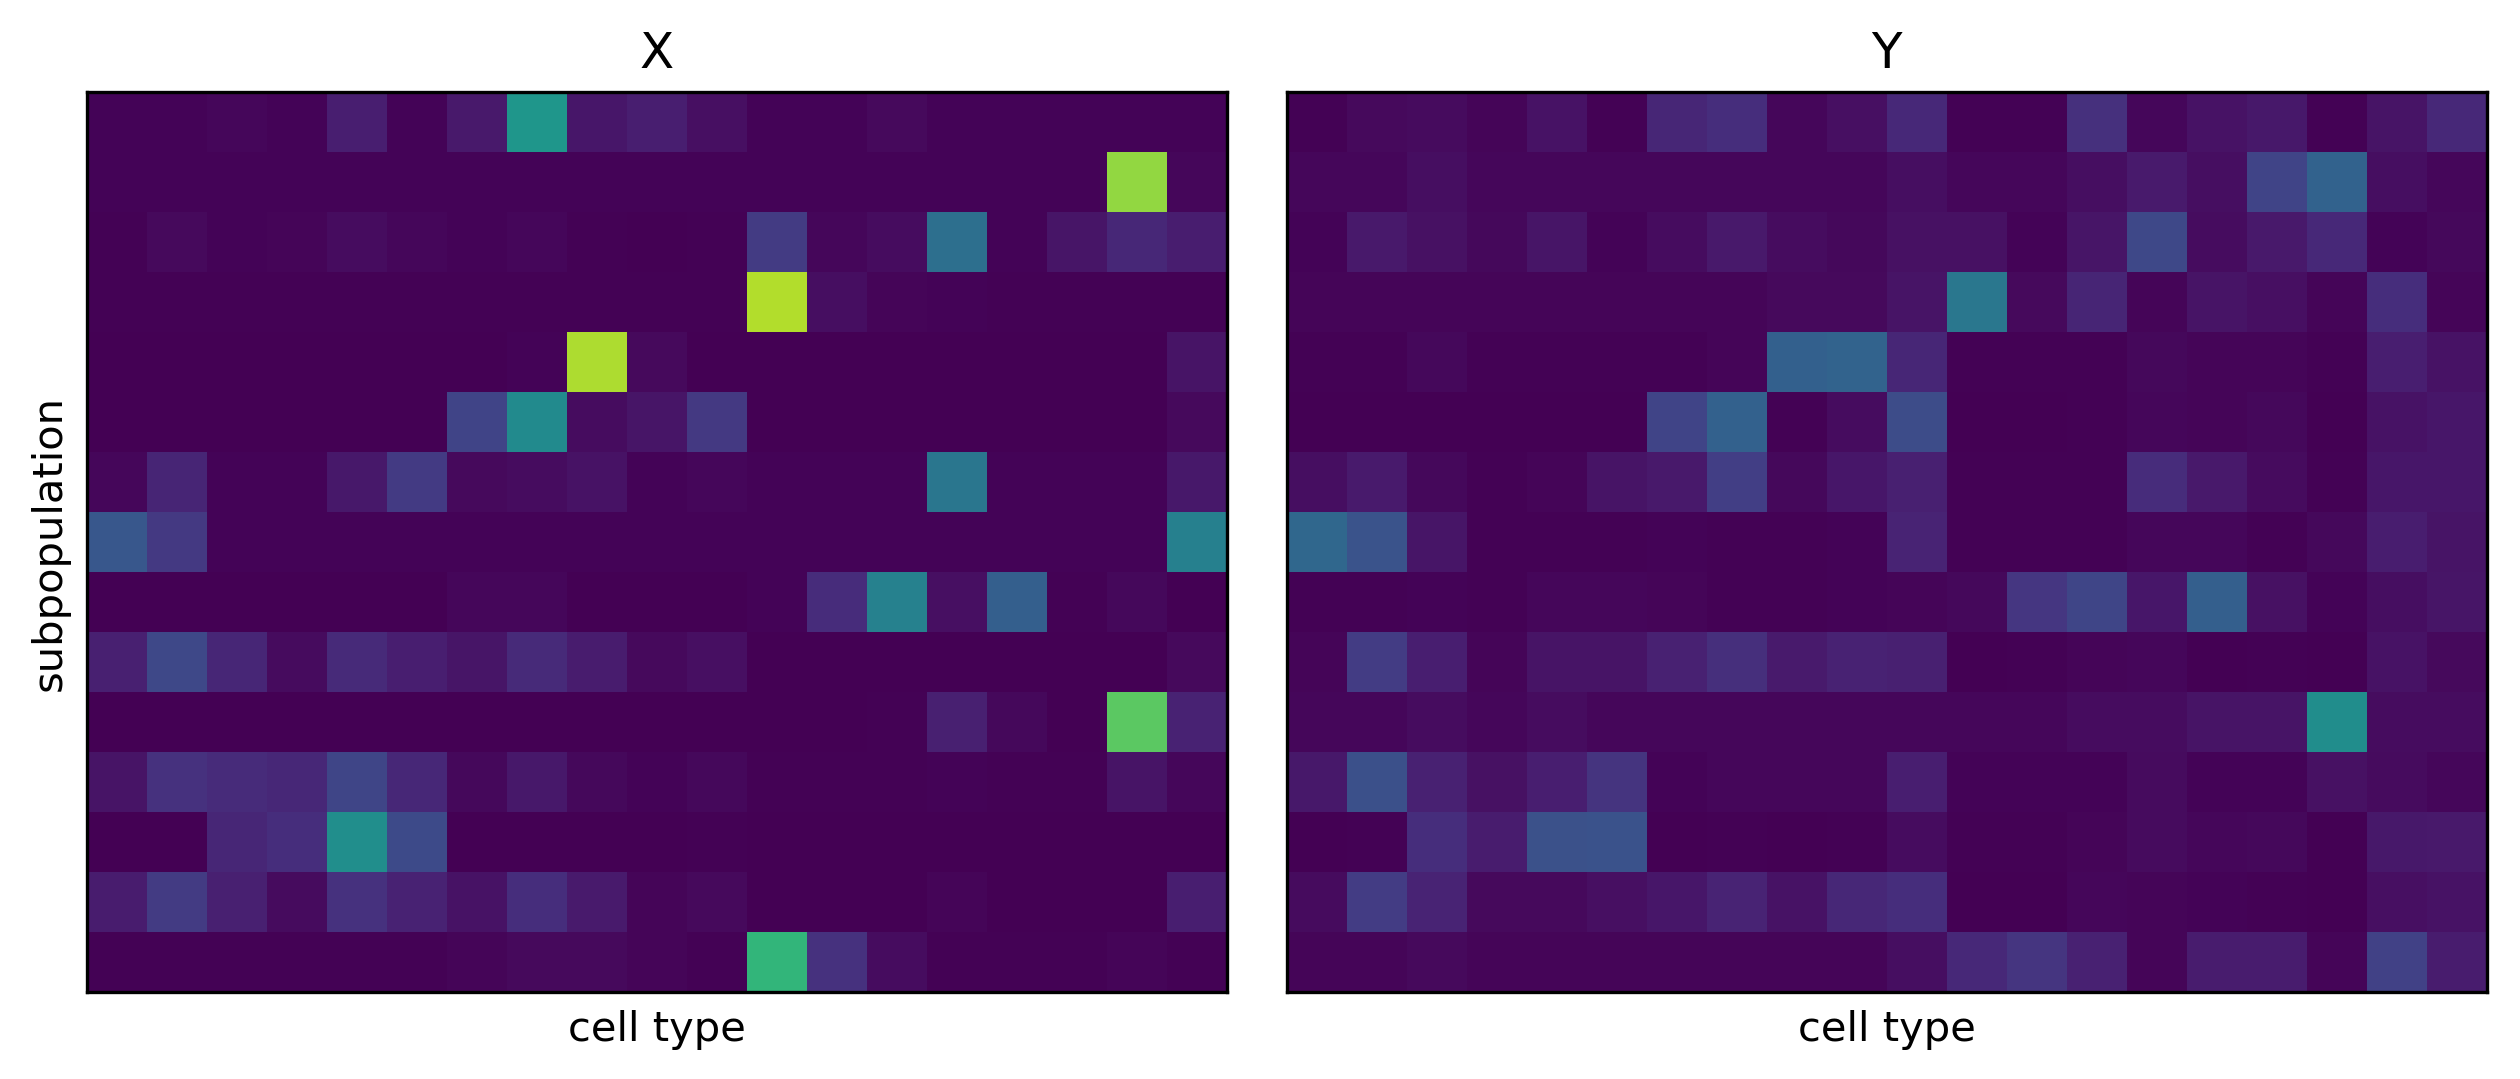
\includegraphics[width=.5\textheight]{../images/plxy}
\hfill{}

\caption{Input: two tables.  The Allen Institute had access to various cre/lox cell selection techniques.  Each technique pulls out a different group of cells.  Once the cells were selected, they were then either subjected to technique I technique II (`patch').  Technique I gives a very complete analysis of the gene expression of the cell.  Technique II gives a less complete analysis, but yields additional electrophysiological data that may be of interest.  For each subpopulation and each technique, data was gathered to estimate the distribution of different cell-types.  These are shown above.  Each column corresponds to a different cell-type.  Each row corresponds to a different subpopulation.  Each entry gives the proportion of a particular cell-type found within a particular population, according to a particular technique.  If the two methods were perfectly calibrated, we would expect the two tables to look identical.  \label{fig:alleninput}}
\end{figure}

\subsection{Background}

Our motivation for this problem arose from looking at Allen Institute cell-type assignment of cells, performed using two different experimental techniques (also called experimental ``modalities'').  Each modality would take a cell and determine what ``type'' of cell it was.  However, as part of that process it would destroy the cell.

Best efforts were made to use biological intuition to calibrate the methods.  For example, if a cell was designated as ``Lamp5 Egln3\_1'' celltype using one method, the hope was that it would also be given the same designation if it was processed using the other method.  The two methods were designed by scientists to achieve this goal.  However, each method has its own biases and errors, and it was not obvious whether this effort was successful.  In particular, it seemed clear that in some cases cells labelled one way with one method would get labelled another way with another method, but it was not clear how often this occurred.  

Fortunately, there was a kind of information that seemed like it might help determine whether the two methods were properly calibrated: sub-populations.  Using a cre/lox system (cf.\ \citep{tasic2017shared}) they were able to pick out specific, overlapping subpopulations of neurons.  Each subpopulation was expected to contain different proportions of the different cell-types.  For each subpopulation and each method, many specimens were sampled and their cell-types determined.  If the methods were perfectly calibrated, we would expect that both methods would yield the same distribution of cell-types in each subpopulation.  

Towards this effort, data was collected for each subpopulation and each method.  The result of this process was two tables, shown in Figure \ref{fig:alleninput}.  Perhaps not surprisingly, it was found that the distribution of cell-types appeared different under the two modalities.  In fact, in one of the methods some of the cells were designated as ``unknown,'' so even the set of cell-types was not the same between the two groups.  Clearly the methods were not perfectly calibrated -- but how big of a problem was it?  It is not obvious to know just by staring at Figure \ref{fig:alleninput}.  A more quantitative method was needed.  

\subsection{Estimation}

The first step of the Markov Link Method was simply to estimate the calibration $q^*$.  Taking $\kappa=.1$, we obtained a calibration found in Figure \ref{fig:allenout}.  While this result seemed to generally suggest the methods were well-calibrated, there are some striking divergences.  For example, this calibration suggests a that celltypes designated as celltype ``10'' in one method are actually quite likely to be designated as celltype ``7'' in the other technique.  Both celltypes are associated with similar neuronal types with high expression of somatostatin.  However, type ``10'' is associated with genes such as `C1ql3,' `Chodl,'  and `Nts,' whereas type ``7'' is associated with `Etv1' and `Myh8.'  

Notice that there are several fundamentally different reasons we could see these kinds of miscalibrations:

\begin{itemize}
    \item The methods are actually miscalibrated.
    \item The subpopulations were unevenly sampled.  It may be that certain techniques tend to cause cell-death in certain cell-types more than others.  These cells are then discarded from the data.  If this process is different between the two techniques, it could have an important impact on the calibration estimated here.
    \item The calibration was poorly estimated.
\end{itemize}

It is to the third point we now turn.

\subsection{Criticism}

TODO:
\begin{enumerate}
\item Nonparametric bootstrap (avg distance 0.66, Figure \ref{fig:nonparametricbootstrap})
\item Parametric bootstrap (avg distance .74, Figure \ref{fig:parametricbootstrap})
\item Held out likelihood (2.21 nats vs our method 2.14 nats)
\item RUX samples (avg distance .16, Figure \ref{fig:ruxsamples})
\item Uniform samples (avg distance .02, Figure \ref{fig:uniformsamples})
\end{enumerate}

\begin{figure}
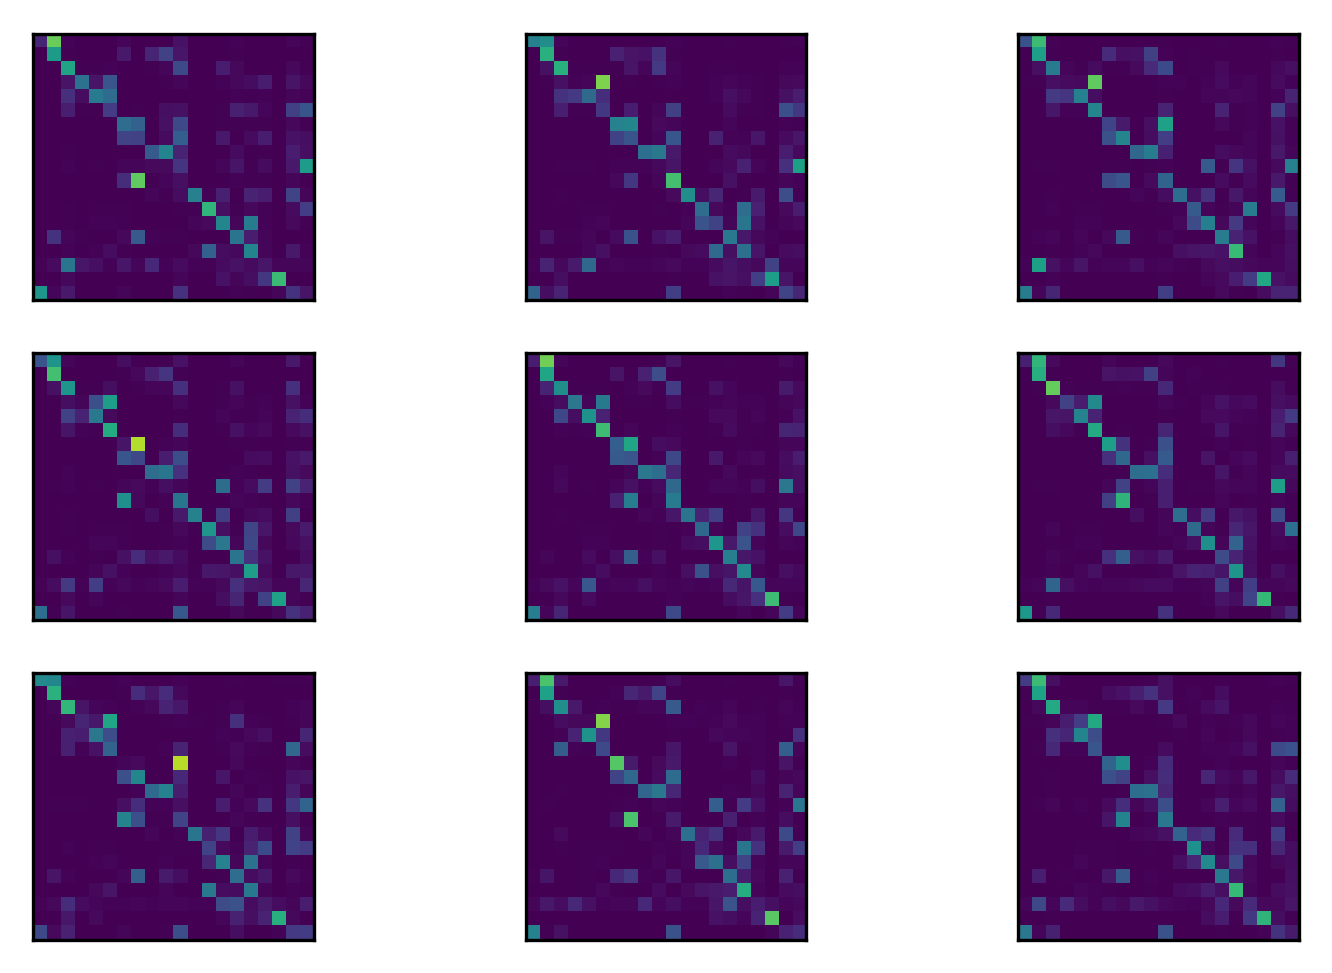
\includegraphics[width=0.8\textwidth]{../images/nonparametricbootstrap}
\caption{Nonparametric bootstrap.\label{fig:nonparametricbootstrap}}
\end{figure}

\begin{figure}
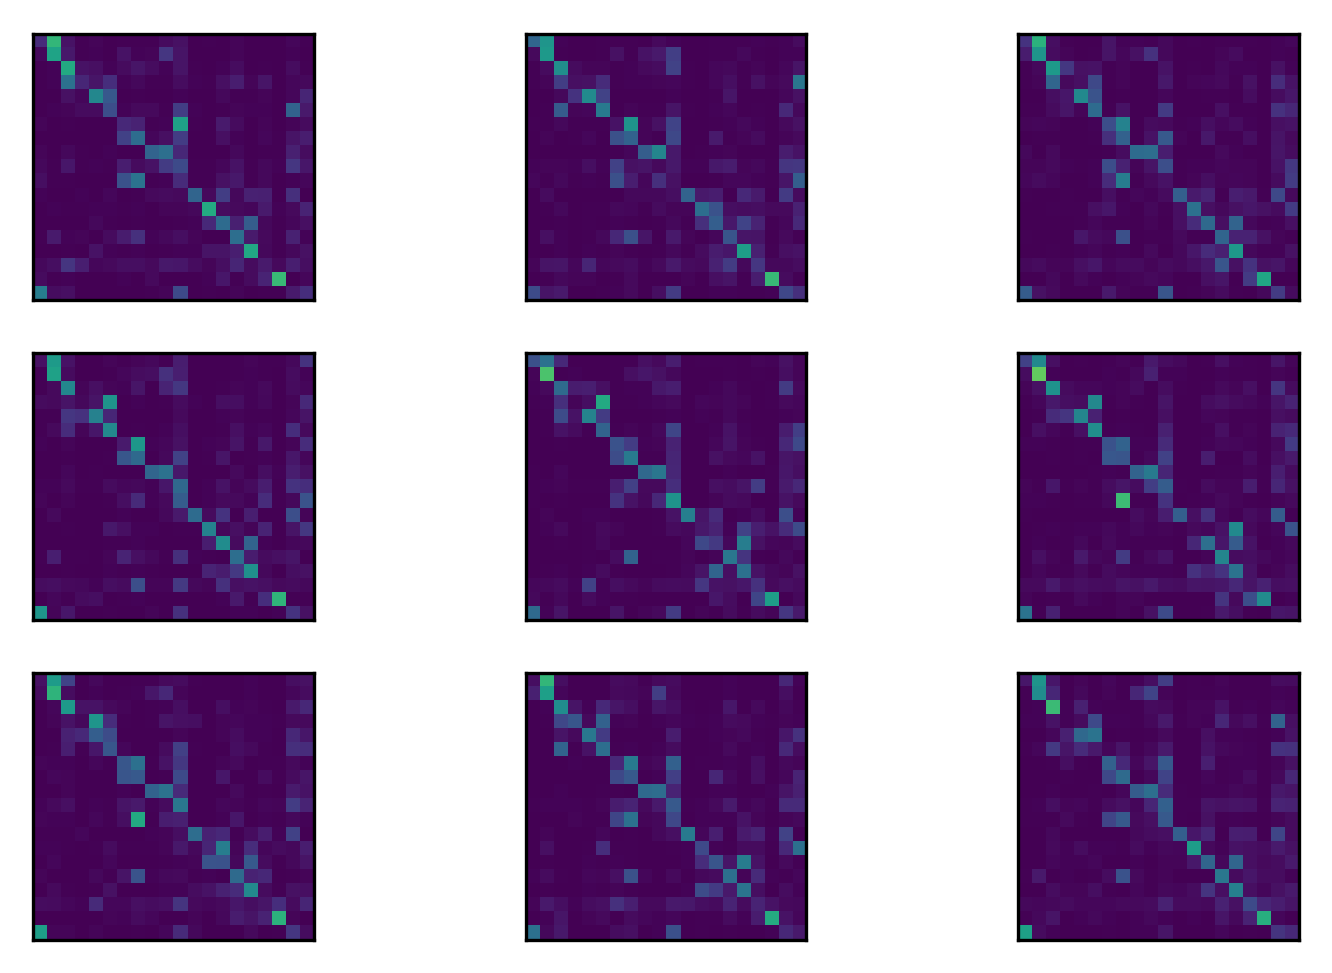
\includegraphics[width=0.8\textwidth]{../images/parametricbootstrap}
\caption{Parametric bootstrap.\label{fig:parametricbootstrap}}
\end{figure}

\begin{figure}
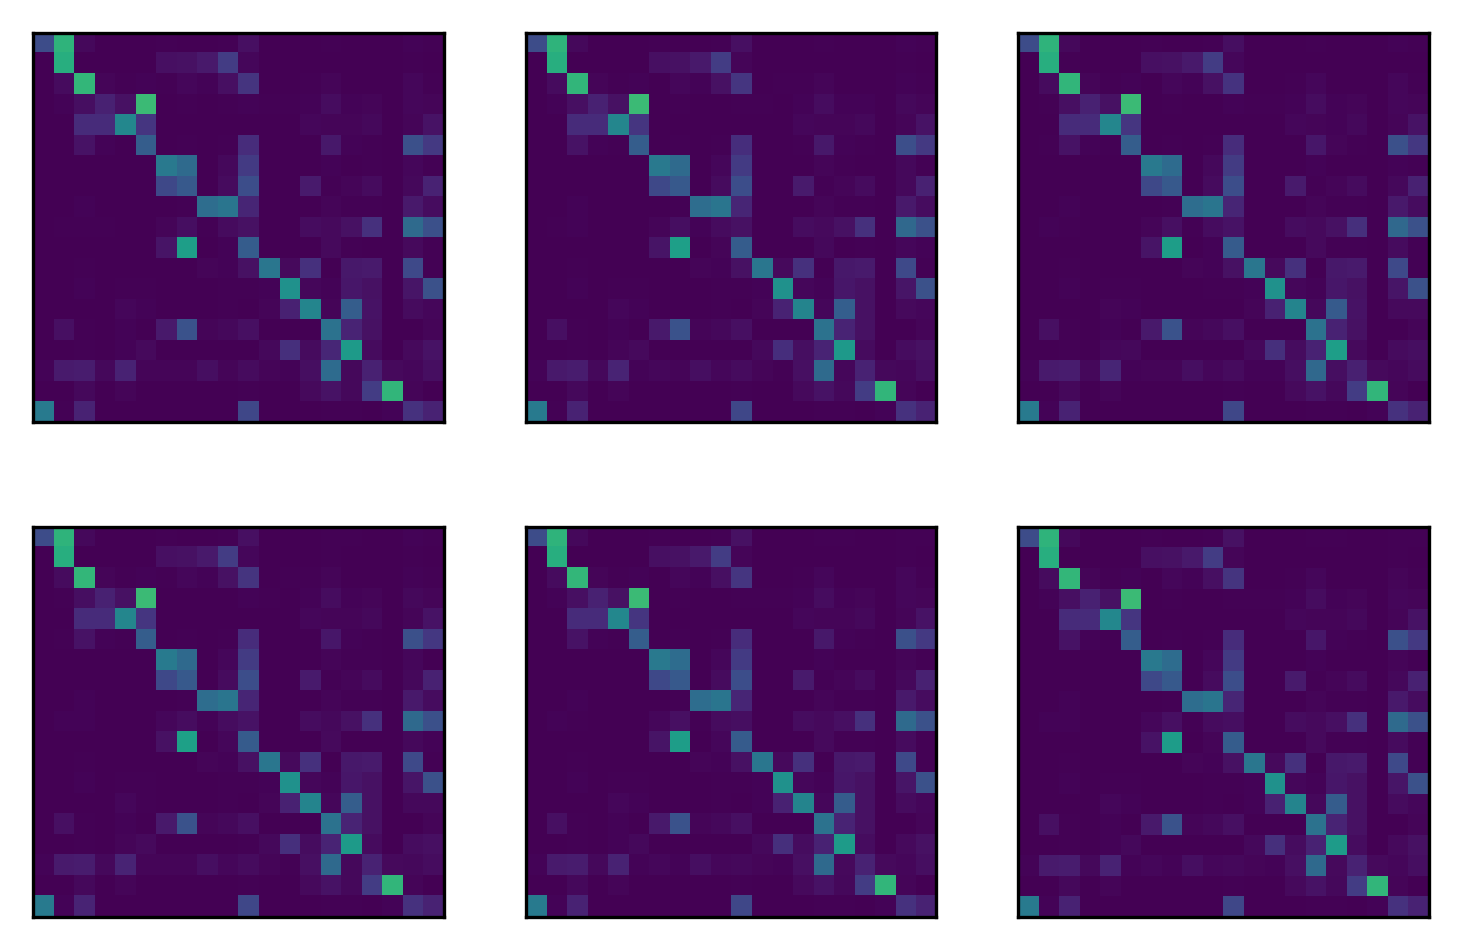
\includegraphics[width=0.8\textwidth]{../images/unif}
\caption{RUX samples.\label{fig:ruxsamples}}
\end{figure}

\begin{figure}
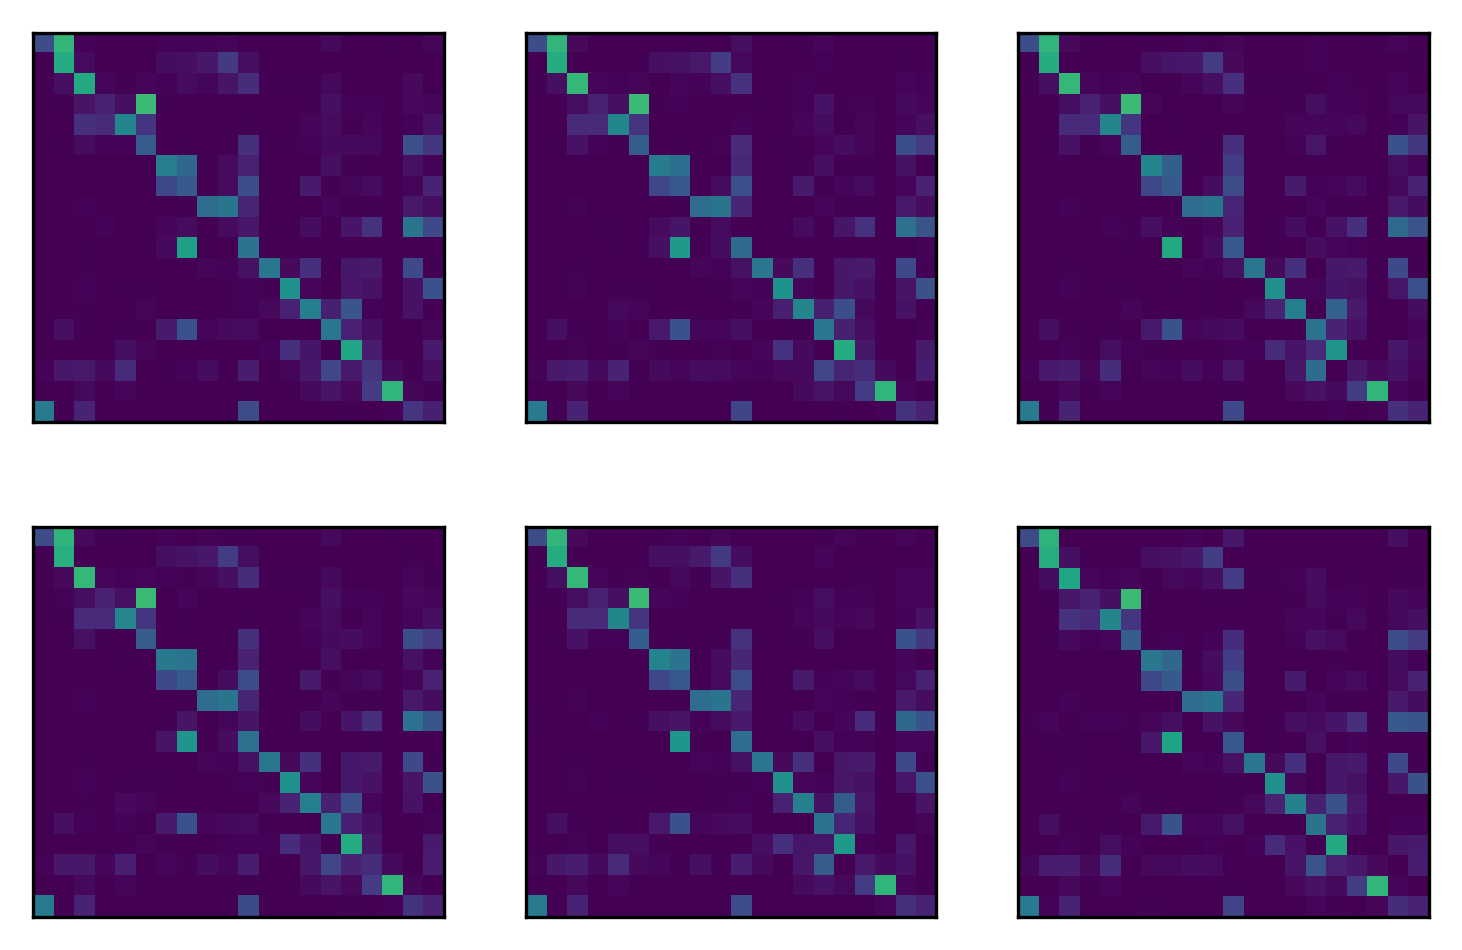
\includegraphics[width=0.8\textwidth]{../images/rux}
\caption{Uniform samples.\label{fig:uniformsamples}}
\end{figure}

\section{Conclusions}

When joint measurement is impossible, it can be difficult to calibrate two methods against each other or understand how they may be related.  Here we show that a simple Markov assumption can make it possible to actually learn quite a lot.  Although the exact relationship may not be identifiable, a polytope of possible relationships can be identified, and this polytope may in fact be quite small indeed.  By exploring this polytope, we can understand what we know -- and what we don't know -- about the relationship between measurements.

The Markov assumption is of course not the only one that we could have used, and may not be valid in every case.  For example, it has been speculated that some cell types tend to die more often in one experimental modality than another, and these cells are not part of the data.  This violates our assumptions.  However, assuming this death rate can be roughly measured, it can be adjusted for, yielding a different but equally meaningful assumption about the data.  Moreover, if this method yields bizarre results, it may give useful clues as to exactly how cell death may happen differently in the two modalities.

Once we accept that what we're interested in may not be fully identifiable, any of a wide variety of assumptions can help us obtain practical bounds.  Although we may not be able to learn exactly what we want, we can learn a set of possibilities.  By probing this set carefully with uniform samplers and extremal tests, we can learn what the data actually has to say and what experiments we need to do to learn more.  

\bibliographystyle{unsrt}
\bibliography{refs}

\appendix

\section{Dikin sampler}

\label{sec:dikin}

Consider a convex polytope $T=\{x:\ Ax\leq b\}$.  We have implemented a method for sampling from this polytope, based on the paper \citep{kannan2012random}.  This method makes use of the Dikin ellipsoids, $E(x)$.  For any $x$, these are defined by 

\begin{itemize}
    \item Computing the distance from $x$ to each facet of the polytope, i.e. $d_i = b_i - \sum_j A_{ij} X_j$.
    \item Constructing $\tilde A$ as $\tilde A_{ij} = A_{ij} / d_i$.
    \item Define $E(x) = \{y:\ |\tilde A (X-y)|\leq 1\}$.  
\end{itemize}

We can use these ellpsoids to efficiently sample the polytope $T$.    At each step, we have some point $X\in T$, and we would to use this point to obtain a new sample $Y$, such that by iterating this process we asymptotically obtain samples which are uniform in $T$.  Here is how we use $X$ to get $Y$:

\begin{algorithm}[H]
 \KwData{A point $X\in T$}
 \KwResult{A point $Y\in T$}
 \vspace{.1in}
  Sample a proposal $\tilde Y$, uniformly from $E(X)$\;
    \eIf{$X \in E(\tilde Y)$}{
        Sample $U \sim \mathrm{Uniform}[0,1]$\;
        \eIf{$U \leq \mathrm{Vol}(E(X))/\mathrm{Vol}(E(\tilde Y)) \leq 1$}{
            Let $Y \gets \tilde Y$\;
        }{
            Let $Y \gets X$\;
        }
    }{
        Let $Y\gets X$\;
    }
 \caption{Dikin sampler step}
\end{algorithm}

It is easy to show that the stationary distribution of the Markov chain found by iterating these Dikin sampler steps is indeed uniform on $T$.  To ensure an numerically robust method in the face of high-dimensional and nearly degenerate matrices, we take the following approach to robustly sampling from the ellipsoid:

\begin{algorithm}[H]
 \KwData{An $n\times m$ matrix $\tilde A$}
 \KwResult{A point $X$ sampled uniformly from $\{x:\ |Ax|\leq 1\}$}
 \vspace{.1in}
  Sample $Z$ as an $n$-dimensional normal variables vector\;
  Let $X$ denote the solution to the least squares problem $\min_x|\tilde Ax - Z|$\;
  Normalize $X$ by $X \gets X/|\tilde AX|$\;
  Sample $U \sim \mathrm{Uniform}[0,1]$\;
  Scale $X$ by $X \gets X \times U^{1/m}$\;
 \caption{Ellipsoid sampler}
\end{algorithm}


\section{Proof of the theorem}

\label{sec:proof}

For the benefit of the reader, we here repeat the statement of our theorem in more explicit terms.  

\begin{itemize}
\item Let $\UN{\cdot}$ denote the uniform norm (i.e.\ the maximum absolute value) and $\EN{\cdot}$ denote the Euclidean norm (i.e.\ the square root of the sum of the squares).  In the case of matrices, this Euclidean norm goes by the name of the Frobenius norm.  Recall that in this norm matrices satisfy a Cauchy-Schwarz like equality, $\EN{pq}\leq\EN{p}\EN{q}$.  Also recall that $\UN{a} \leq EN{a} \leq \sqrt{n}\UN{a}$ where $n$ is the number of entries in $a$.
\item Let $T_{a,b}$ denote the transition matrix polytope, i.e. the set of $a\times b$ matrices whose rows sum to 1 and whose entries are all positive.
\item Let $|\Omega_\ell|,|\Omega_X|,|\Omega_Y| \in \mathbb{N}$.
\item Let $p^*\in T_{|\Omega_\ell|,|\Omega_X|}$.
\item Let $q^*\in T_{|\Omega_X|,|\Omega_Y|}$.
\item We require the matrix $q^*$ has strictly positive entries, $q^*_{xy}\geq c>0$.
\item We require that the rows of $p^*$ are linearly independent.
\item Let $\hat p$ denote an empirical transition matrix drawn by obtaining $N_{X,\ell}$ samples for each row of $p^*$, i.e. we have samples $(\ell_1,X_1) \cdots (\ell_1,X_n)$ such that $\mathbb{P}(X_i=x) = p^*_{\ell_i,x}$, $N_{X,\ell}=\sum_{i=1}^n \mathbb{I}_{\ell_i=\ell}$, and $\hat p_{\ell x} = \sum_{i=1}^n \mathbb{I}_{X_i=x,\ell_i=\ell} / N_{X,\ell}$. 
\item Let $\hat h$ denote an empirical transition matrix drawn by obtainin $N_{Y,\ell}$ samples for each row of $h^*=p^*q^*$.  
\end{itemize}

Now fix any $\kappa>0$.  Let
\begin{align}
\hat q = \argmax_q \left(\sum_\ell N_{Y,\ell}\sum_{y}\hat h(y|\ell)\log\left(\sum_{x}\hat p(x|\ell)q(y|x)\right) + \kappa \sum_{xy} \log q(y|x)\right)\label{eq:mindef}
\end{align}
and $\hat \Theta=\{q:\ \hat p\hat q=\hat pq\} \cap T_{|\Omega_X|,|\Omega_Y|}$.  
\vspace{.1in}
\begin{thm}
If $N_{X,\ell},N_{Y,\ell}\rightarrow \infty$ in such a way that $N_{Y,\ell'}/\sum_{\ell}N_{Y,\ell} \geq \rho>0$ for each $\ell'$, then $\inf_{q\in \hat\Theta} \UN{q^*-q}\rightarrow 0$ in probability.
\end{thm}

\begin{proof}
It is well-known that $\hat p\rightarrow p^*$ in probability (in both the uniform or the Euclidean norm, which are of course equivalent in this case).  It is easy to see that the same goes for $\hat p\hat q\rightarrow h^*$ (see Lemma \ref{lem:easyconsistency}).  Thus, intuitively, the difficulty is this: by allowing ourselves to ensure $\UN{\hat p - p^*},\EN{\hat p - p^*},\UN{\hat p\hat q - h^*},\EN{\hat p\hat q - h^*}$ sufficiently small, can we find some $\tilde q\in \hat \Theta$ so that $\UN{\tilde q - q^*}$ is arbitrarily small?  It turns out we can.

Recall that $c>0$ is the smallest value of $q^*_{xy}$.  Fix any $\epsilon<c, p^*,q^*$.  Let the right inverse of a matrix be defined by $a^\dagger \triangleq a^T (aa^T)^{-1}$.  Note that since $p^*$ has linearly independent rows, this is well-defined and continuous in a small neighborhood around $p^*$.  Let $M=\EN{(p^*)^\dagger}$.  Find $\delta$ small enough so that if $\UN{p-p^*}<\delta$ then $\EN{p^\dagger}<2M$.  Taking a further smaller $\delta$ if necessary, ensure that if $\UN{p^*-p}<\delta$ then $\EN{p^*-p}$ is less than $\epsilon / 4M\sqrt{|\Omega_X||\Omega_Y|}$.  
Now fix any $\hat p,\hat q$ with $\UN{\hat p-p^*}<\delta$ and $\EN{\hat p \hat q - p^*q^*}<\epsilon/4M$.  Take
\[
\tilde q = q^* + \hat p^\dagger \hat p (\hat q - q^*)
\] 
Then we make the following observations:
\begin{itemize}
  \item Let us compute $\EN{\tilde q -q^*}$. We have
   \begin{align*}
   \EN{\tilde q -q^*} &= \EN{\hat p^\dagger \hat p (\hat q - q^*)} \leq 2M \EN{\hat p \hat q - \hat p q^*} \\
        &\leq 2M \EN{\hat p \hat q - p^* q^*} + 2M\EN{(p^* - \hat p)q^*}\\
        &\leq 2M \frac{\epsilon}{4M} + \frac{2M\epsilon}{4M\sqrt{|\Omega_X||\Omega_Y|}}\sqrt{|\Omega_X||\Omega_Y|}\UN{q^*} \leq \epsilon 
   \end{align*}
  \item $\hat p \tilde q = \hat p q^* + \hat p \hat q - \hat p q^* = \hat p \hat q$
  \item The rows of $\tilde q$ sum to 1.  This is easy to see, because the rows of $q^*$ sum to 1 and the rows of $\hat q$ sum to 1, and so $\tilde q \mathbf{1} = q^* \mathbf{1} + \hat p^\dagger \hat p (\hat q - q^*) \mathbf{1} = \mathbf{1} + 0$ as desired.
  \item The entries of $\tilde q$ are positive.   Indeed, the the smallest value of $q^*$ is $c$, and we have already argued that $\UN{\tilde q - q^*}\leq \epsilon$.  Thus the smallest value of $\tilde q$ is at least $c-\epsilon$, and we have required $\epsilon<c$.  
\end{itemize}
Thus $\UN{\tilde q - q^*}<\epsilon$ and $\tilde q \in \hat \Theta$.  

In conclusion, we see that by taking $\hat p$ sufficiently close to $p^*$ and $\hat p \hat q$ sufficiently close to $p^*q^*$, we can ensure that the set $\hat \Theta$ contains a close which is arbitrarily close to the true $q^*$.  Since $\hat p$ and $\hat p \hat q$ are themselves consistent estimators, this completes the proof.
\end{proof}

\begin{lem}
\label{lem:easyconsistency} If $N_{X,\ell},N_{Y,\ell}\rightarrow \infty$ in such a way that $N_{Y,\ell'}/\sum_{\ell}N_{Y,\ell} \geq \rho>0$ for each $\ell'$, then $\UN{p^*q^*-\hat p\hat q},\EN{p^*q^*-\hat p\hat q}\rightarrow 0$ in probability.
\end{lem}
\begin{proof}
Our first task is to make a short study of the continuity of KL divergences on categorical distributions when the probabilities are bounded away from zero.  Recall that we have insisted $q^*_{xy}\geq c>0$ for every $x,y$ -- and this also means $(pq^*)_{\ell y}\geq c$ for every $\ell,y$, since each row of $p$ is itself a probability distribution.  Moreover, observe that the KL-divergence on $|\Omega_Y|$-dimensional distributions, $\kldiv{\hat r}{\tilde r} \triangleq \sum_{y} \hat r_y \log \hat r_y / \tilde r_y$, is \emph{uniformly} continuous on the space of such distributions whose minimum probability is greater than any fixed positive constant.   It follows that the map $h,p,q \mapsto D(h_\ell||(pq)_\ell)$ is also uniformly continuous on a space where $h$ and $q$ are strictly greater than some fixed positive constant.   

With this in hand, the remainder of the proof follows naturally, using the well-known results that empirical distributions are consistent, i.e.\ $\hat p \rightarrow p^*$ and $\hat h \rightarrow p^*q^*$ in probability.

Fix any $\epsilon,\pi$.  Let $\delta$ the modulus of continuity in the norm $\UN{\cdot}$ at level $\epsilon\rho$ for the map $h,p,q \mapsto \kldiv{h_\ell}{(pq)_\ell}$ restricted to the domain where $h,q>c/2$.  Select $N$ large enough so that $\frac{1}{N_{Y,\ell}} \kappa |\Omega_X||\Omega_Y| \log \frac{1}{c} < \epsilon$ for each $\ell$ and so that with probability at least $\pi$ we have that $\hat h,\hat p$ so that $\UN{\hat h-p^*q^*},\UN{\hat p-p^*}\leq \delta,\UN{\hat h - p^*q^*}<c/2$. Then, with probability $\pi$, we must have
%
\begin{align*}
|\kldiv{\hat h_\ell}{(\hat p \hat q)_\ell} - \kldiv{h^*_\ell}{(\hat p \hat q)_\ell}| \leq \rho \epsilon \\
\kldiv{\hat h_\ell}{(\hat p q^*)_\ell} = |\kldiv{\hat h_\ell}{(\hat p q^*)_\ell} - \kldiv{(p^*q^*)_\ell}{(p^* q^*)_\ell}| \leq \rho\epsilon 
\end{align*}
%
Now, since $\hat q$ is defined as the maximizer of a certain quantity (Equation \ref{eq:mindef}), we may be sure that it is greater than the same quantity evaluated at $q=q^*$.  That is,
%
\begin{align*}
0 \leq& \sum_\ell N_{Y,\ell}\sum_{y}\hat h(y|\ell)\log\frac{\sum_{x}\hat p(x|\ell)\hat q(y|x)}{\sum_{x}\hat p(x|\ell)q^*(y|x)} + \kappa \sum_{xy} \log \frac{\hat q(y|x)}{q^*(y|x)}\\
 =& \sum_\ell N_{Y,\ell}\left(\kldiv{\hat h_\ell}{(\hat pq^*)_\ell} - \kldiv{\hat h_\ell}{(\hat p\hat q)_\ell}\right) + \kappa \sum_{xy} \log \frac{\hat q(y|x)}{q^*(y|x))}
\end{align*}
%
Applying our continuity results, it follows that
%
\begin{gather*}
 \sum_\ell N_{Y,\ell}\left(\kldiv{\hat h^*_\ell}{(\hat p\hat q)_\ell}\right)  \leq 2\left(\sum_\ell N_{Y,\ell}\right)\epsilon  + \kappa |\Omega_X||\Omega_Y| \log \frac{1}{c} 
\end{gather*}
%
Note that the left-hand summands are all positive.  So, in particular, it follows that for each $\ell'$, applying the uniformity condition $\rho$, we have
%
\begin{gather*}
\kldiv{\hat h^*_{\ell'}}{(\hat p\hat q)_{\ell'}}  \leq 2\epsilon  + \frac{1}{N_{Y,\ell'}} \kappa |\Omega_X||\Omega_Y| \log \frac{1}{c} \leq 3\epsilon
\end{gather*}

That is, we have shown convergence of probability in the KL sense: for any $\epsilon,\pi$ we can find $N$ high enough so that $\kldiv{\hat h^*_{\ell'}}{(\hat p\hat q)_{\ell'}}<\epsilon$ with at least probability $\pi$.  This, in turn yields convergence in probability in the Euclidean or uniform metrics by Pinsker's inequality. 
\end{proof}

\end{document}






































